\documentclass[11pt,english]{article}
\usepackage[utf8]{inputenc}
\usepackage[T1]{fontenc}
\usepackage{babel}
\usepackage{biblatex}
\addbibresource{bibliography.bib}
\usepackage{graphicx}
\graphicspath{ {./images/} }

% correct bad hyphenation here
\hyphenation{op-tical net-works semi-conduc-tor}
\begin{document}
\title{Use of Model-Driven Development to check for violations of the GDPR}
\author{
  Tijana Lalošević\\
  \texttt{tijana.vdn@gmail.com}
  \and
  Gordana Milosavljević\\
  \texttt{grist@uns.ac.rs}
  \and
  Goran Sladić\\
  \texttt{sladicg@uns.ac.rs }
  \\Faculty of Technical Sciences,\\ University in Novi Sad, Serbia
}


\date{}
\maketitle


\begin{abstract}
The General Data Protection Regulation (GDPR) \cite{gdprRegulation} is a legal regulation on the use, protection and privacy of data issued by the European Union. The GDPR was adopted on 14 April 2016 and became enforceable beginning 25 May 2018. \cite{gdpr} This regulation aims to give individuals control over their data across the European Union and unify laws within the European Union to facilitate international business. This regulation is a mixed blessing. On the one hand, it has brought many benefits to individuals, but also, it has provided many challenges and obstacles to companies and organizations that control or process personal data. Despite unification and centralization of law regulation, there is no universal software solution for checking GDPR compliance. Therefore, to overcome some of the security challenges, companies pay expensive manual checking executed by lawyers or create solutions that do not apply to other organizations and industries. In this paper, we propose a solution in the form of a privacy meta-model, as also, OCL validations \cite{ocl} which provides automatical checking for violations of the first fifty arts of the GDPR. Besides, we will present usage of this meta-model on an example of a bank and plan of future development.
\end{abstract}

\section{Introduction}

\quad The development of technology and the discovery of new technologies have brought extraordinary changes in many living fields and the growth of living standards. These innovations are creating new goods that are becoming a source of demand for more and more people. Thus, the data stood out as the "gold" of the 21st century. As such, they caused more and more frequent abuses. One of the many problems is leakage of sensitive information, their sale on the black market, modifications, intellectual property thefts, and many others. Because of that reason, their use had to be legally regulated. Also, there was a need to introduce information security management. Information security risk management (ISRM) is the primary means by which organizations preserve the confidentiality, integrity and availability of information resources. \cite{WEBB20141} Digitalization and globalization have erased international borders and enabled the rapid growth and development of international business. Increased business movements have led to the problem of legislative inconsistencies between the countries in which it operates. This gap between regulations has made a place for many data thefts, resale and other abuses. To overcome this problem, the European Union adopted a legal framework, the GDPR, which unified privacy management and data protection. On the business side, this regulation caused a great deal of difficulty as companies had to adjust their business to the new rules in a brief period.
\newline \quad Many surveys conducted to determine how ready the market is for the new regulations. Based on Isaca survey \cite{isaca} the top five advantages related to GDPR compliance are:
\begin{itemize}
  \item Data discovery and mapping (59 per cent)
  \item Prioritizing GDPR compliance among other business priorities (47 per cent)
  \item Organizational education and change programs (45 per cent)
  \item Ensuring cross-departmental collaboration and buy-in (42 per cent)
  \item Preparation for data subject access or deletion requests (37 per cent).
\end{itemize}
\quad The Lipswitch survey \cite{lipswitch} has given the following results similar to the first survey. This survey reveals that 52 per cent of the examined companies admitted they were not ready to apply the GDPR, besides 35 per cent confessed to not knowing whether their IT policies and process were up to the job. Seo, Kim, Park and Lee \cite{8190804} have analyzed the economic impact on IoT under
GDPR. They examine which parts of Gordon and Loeb’s defined costs \cite{gordon2002economics} are expected to change due to GDPR, as is shown in Figure 1. They estimated the company’s cost for each of these four types, as is shown in Figure 2.
\begin{figure}[htp]
    \centering
    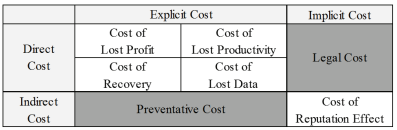
\includegraphics[width=6cm]{costs}
    \caption{Gordon and Loeb Model’s Cost that GDPR affects}
    \label{fig:costs}
\end{figure}
\begin{figure}[htp]
    \centering
    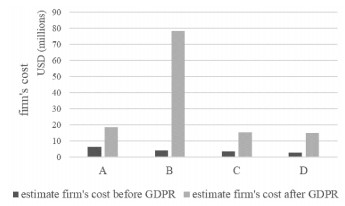
\includegraphics[width=6cm]{comparation}
    \caption{Comparison of company’s cost before and after GDPR}
    \label{fig:comparation}
\end{figure}
\newline These results are not unexpected, as it is the main cause for that is a lack of a single comprehensive solution that would be applicable and easy to integrate into all technologies. The secondary cause was a misunderstanding of terms and expressions which have come with the GDPR. Therefore companies are most often forced to pay legal experts to study their business ecosystem. After that, based on those studies, the IT team designs a unique solution for their information system. The whole process is slow, expensive, and errors prone. \newline This paper aims to define a universal meta-model that is close to natural language that can describe the real scenarios of using personal data in the information system and check whether their usage follows the GDPR. To achieve this goal, we used Model-Driven Engineering (MDE) technologies \cite{mde}, such as UML \cite{uml} and Object Constraint Language (OCL). After that, we will analyze the expressiveness of the meta-model and the usability of OCL validations on the example of the bank case study. Finally, as it is the first step towards easy integration with software solutions and automatical verifying compliance of business processes to the GDPR, we will introduce our strategy for future development. \newline The GDPR is considered the toughest and rigorous privacy and security law in the world.  The fact that it includes all manipulations over the data manifests its complexity. Starting with data collection, storage and transformation, transport, processing and ends with stop processing. It places special emphasis on the data owner and the role he assumes in the data processing. The data owner is the only one who can manage the data, introducing terms such as complaint, withdrawal of consent and request for the erasure. We can see how comprehensive the GDPR is in that it covers all previously adopted regulations and safety standards. So in the overview of the works, we will also consider solutions that rely on previously adopted regulations. \newline The structure of the paper is as follows. In the second section, 'Related Work', we provide the related work. In the third section, ‘Privacy meta-model’, we present our meta-model with accompanying OCL validations. After that, in section ‘Case study’, we demonstrate the usage of the meta-model on the example of a bank case study. In section ‘Discussion’,  we discuss the results and limitations of the study. Finally, in section ‘Conclusion’, the paper has been concluded, and some future development has proposed.
\section{Related work}
Before the appearance of the GDPR, many different regulations and laws were in force. As we already mentioned before, the GDPR covers all of these regulations.  There have been many proposed solutions that deal with compliance of business processes with applicable legislation. As these solutions had been in use for many years and showed as suitable for usage, we decided to use them in our research.
\subsection{Earlier regulations}
Since digitalization prevailed, the data became more accessible, so the software became more susceptible to software attacks. In order to define a certain standard for data protection, states regulated them by law. Due to the large amount of personal data they handle, the IoT \cite{iot} and health systems have stood out as the most attractive targets for hacker attacks. Considering the nature of these systems, they required automation of processing and collection of data.  According to this, most of the previous research has been concerned with finding solutions for them.\newline The first hurdle the industry faced was data encryption. Hence, Ding and Klein \cite{encryptionLevel} propose a novel model-driven application-level encryption solution to protect the privacy and confidentiality of health data. They suggest the cooperation of domain experts, who specify sensitive data, and security experts, who determine cryptographic parameters, thus creating the security configuration. After that, the code generator generates code and configuration artefacts to control the encryption and decryption logic. On the other side, Amato, Flora, and Moscato suggest a different approach. In their first paper \cite{6245777}, they introduced MetaMORP(h)OSY methodology and framework. Then, they present the solution \cite{amato2015model} based on lifecycle validation. They extend the MetaMORP(h)OSY modelling profile to explicitly consider privacy requirements for data. Authors specialize the stereotype for every role in the health system. After that, they create a data lifecycle with predefined states containing semantics. Then, they implement a translation algorithm to perform verification at every lifecycle step. \newline Rahmouni, Solomonides, Mont and Shiu \cite{rahmouni2011model} were the first to recognize the problem with the different rules governing privacy protection. Their proposed solution is an ontology-plus-rules based approach to privacy decision support. Their target group was health systems across Europe. Their solution uses the Web Ontology Language (OWL) \cite{owl} to represent privacy rules in the context of medical data. Choosing the OWL has several advantages. It gives the possibility of overlapping model concepts, even when legally objects use a different naming convention for the same resource. However, the OWL cannot solve complex legal rules based on if-else logic. In this case, they used the Semantic Web Rule Language (SWRL) \cite{swrl} for them. This solution has been contemporary and comprehensive. They were among the first to recognize the concept of consent and the purposes of data processing. Through evaluating phase, they focus on the health system from states which are part of the EU, like the UK, Italy and France. The most relevant requirement was patient consent for two critical phases of the data lifecycle, as uploading the data and sharing the data.
\subsection{GDPR}
One of the significant technic breakthrough after the discovery of the Internet was cloud computing. Cloud computing presents the delivery of different resources as applications, data storage and databases through the Internet. On the one hand, it proves a new level of flexibility and scalability. On the other hand, it brings new security and privacy challenges. \newline Opara, Song, Cho and Chung addressed these challenges in an extraordinary way. They introduce CERBERUS \cite{opara2019representing}, a framework for representing multi-cloud security and privacy policies and detecting potential problems in the security policies. CERBERUS consists of DSL, which is extremely easy to use and close to natural language. What makes this DSL simple is the use of pronouns and adjectives, such as who, why, when and so on. Precisely because of this, it is easy to understand even for people who know nothing about the legislation or privacy models. It uses two categories of security policies, authorization (A) and obligation (O). After creating a specific instance, it looks for inconsistencies in access rights and thus validates the model. Barati and Rana \cite{barati2020tracking} represent a solution for cloud privacy that uses blockchain technology for auditing purpose. They created the GDPR Contract Factory. This factory generates four smart contracts (compliance, user consent, container and verification contract) that provide the basis for the verification of actor operations and privileges. Each of these four contracts answers one of four legal questions, which are defined earlier in the paper \cite{corrales2018smart}. 
\begin{itemize}
    \item Legal question L1: relates to the sensitivity of user data. In the GDPR standard, sensitive data consists of information, such as religious or political beliefs, genetic data, biometric data and health-related data.
    \item Legal question L2: checks if cloud services have a user
authentication mechanism.
    \item Legal question L3: verifies the geographical location of a
provider receiving user data.
    \item Legal question L4: checks for Binding Corporate Rules
(BCR) certification of non-European data receivers. The BCR is a code of conduct adopted by a community of multinational companies that want to move user data internationally across various jurisdictions.
\end{itemize}
They evaluate the presented solution on the example of the pharmacy service hosted at a cloud data centre. The disadvantage of this solution is that it is closely related to cloud computing and has a small set of user actions, there are only read, write, transfer and profiling user actions.
Resenje koje se oslanja na rbac u kompu MODELSWARD. Zanimljivo resenje dsl u kompu. Primar jednog dobrog dsla u kompu dialogo.
It is interesting to see the analogy between the and our approach. pa staviti onaj rad model driven gdpr. Zeleli smo da napravimo pojednostavljen dsl koji ce biti lako razumljiv i ljudima koji nisu pravnici. 
\section{Privacy meta-model}
\section{Case study}
\section{Discussion}
\section{Conclusion}
\printbibliography
\end{document}
